\documentclass[tikz, convert = false]{standalone}%

\usepackage[utf8]{inputenx}%  http://ctan.org/pkg/inputenx
% Euler for math | Palatino for rm | Helvetica for ss | Courier for tt
\renewcommand{\rmdefault}{ppl}% rm
\linespread{1.05}% Palatino needs more leading
\usepackage[scaled]{helvet}% ss //  http://ctan.org/pkg/helvet
\usepackage{courier}% tt // http://ctan.org/pkg/courier
\usepackage{eulervm}  %  http://ctan.org/pkg/eulervm
% a better implementation of the euler package (not in gwTeX)
\normalfont%
\usepackage[T1]{fontenc}%  http://ctan.org/pkg/fontenc
\usepackage{textcomp}%  http://ctan.org/pkg/textcomp

\begin{document}
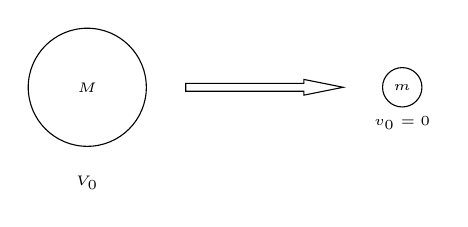
\begin{tikzpicture}
  \draw (0, 0) circle[radius = .75] node[font = \tiny, below] at (0, -1)
  {$V_0$};
  \draw (4, 0) circle[radius = .25] node[font =\tiny, below] at (4, -.25)
  {$v_0 = 0$};

  \node[font = \tiny] at (0, 0) {$M$};
  \node[font = \tiny] at (4, 0) {$m$};

  \draw[xshift = -.25cm] (1.5, .05) -- (3, .05) -- (3, .1) -- (3.5, 0) --
  (3, -.1) -- (3, -.05) -- (1.5, -.05) -- cycle;
\end{tikzpicture}
\end{document}
%%% Local Variables:
%%% mode: latex
%%% TeX-master: t
%%% End:
